\documentclass[ 12pt, a4paper]{article}
\usepackage[ ]{indentfirst}
\usepackage{amssymb}
\usepackage[ ]{pdflscape}
\usepackage[ ]{graphicx}
\usepackage[ ]{booktabs}
\title{Revisão P2\\Construção de Compiladores\\Prof. Bráulio de Mello}
\author{Erickson G. Müller}
\date{11 de junho de 2026}

\begin{document}
\maketitle
\section*{Conteúdos}
	\begin{itemize}
		\item Tradução dirigida por sintaxe
		\item Esquemas de tradução
		\item Gramática de atributos
		\item Esquemas S-atribuídos
		\item Árvores de Sintaxe
		\item Análise Semântica
		\item Geração de código intermediário
		\item Otimização de código
	\end{itemize}
\newpage

\section{Tradução dirigida por sintaxe}
\begin{itemize}
	\item $AS \to $ tradução
	\begin{itemize}
		\item código
			\begin{itemize}
				\item operações básicas
				\item mesmo nível
			\end{itemize}
		\item interpretação
		\item ações semânticas
		\item add dados TS
		\item tratamento de erro
	\end{itemize}
\end{itemize}
	\subsection{Árvore de derivação anotada}

	Atributos associados aos símbolos.\\
	\textbf{Exemplo:}\\
		$D::= var: T$\\
		$T::= real$\\
		$T'::= int$\\
		\\
		Ações semânticas:\\
		$\{$add $TS(var.nome, T.tipo)\}$\\
		$\{T.tipo='r'\}$\\
		$\{T.tipo='i'\}$\\
		\\
		$_{var.nome=x_1}$\\
		$_{T.tipo = 'r'}$\\
		cadeia: $x_1:real$

\begin{verbatim}
	TS
	___________________________________
	| x1, r

\end{verbatim}
	\subsection{Esquemas de tradução}

		Esquemas de tradução é o conjunto de ações semânticas

		Todo tipo de transformação que aconteece no código é uma tradução. (Código alto nível $>$ código temporário 2 operandos $>$ código de máquina), o reconhecimento sintático conduz essa tradução. Toda transformação conduzida pela sintaxe cujas regras estão na GLC é a tradução dirigida por sintaxe.
	\begin{itemize}
		\item extensão da GLC
		\item atributos
			\begin{itemize}
				\item Sintetizados: atributo computado a partir dos valores dos atributos dos filhos do símbolo.
				\item Herdados: atributo computado a partir dos valores dos atributos dos irmãos ou do pai do símbolo.
			\end{itemize}
		\item ações semânticas
		\item grafo de dependência
			\begin{itemize}
				\item ordenação uso atributos
			\end{itemize}
		\item passos
			\begin{itemize}
				\item Análise sintática
				\item Árvore de derivação (anotada)
				\item grafo de dependência
			\end{itemize}
	\end{itemize}
	
	\textbf{Exemplo 2:}\\
	$E::=TR$\\
	$R::= Op$ $T \{$print $(Op.simbolo)\}$ $R|E$\\
	$T::= num$ $\{$print $(num.lexval)\}$\\
	\begin{center}
	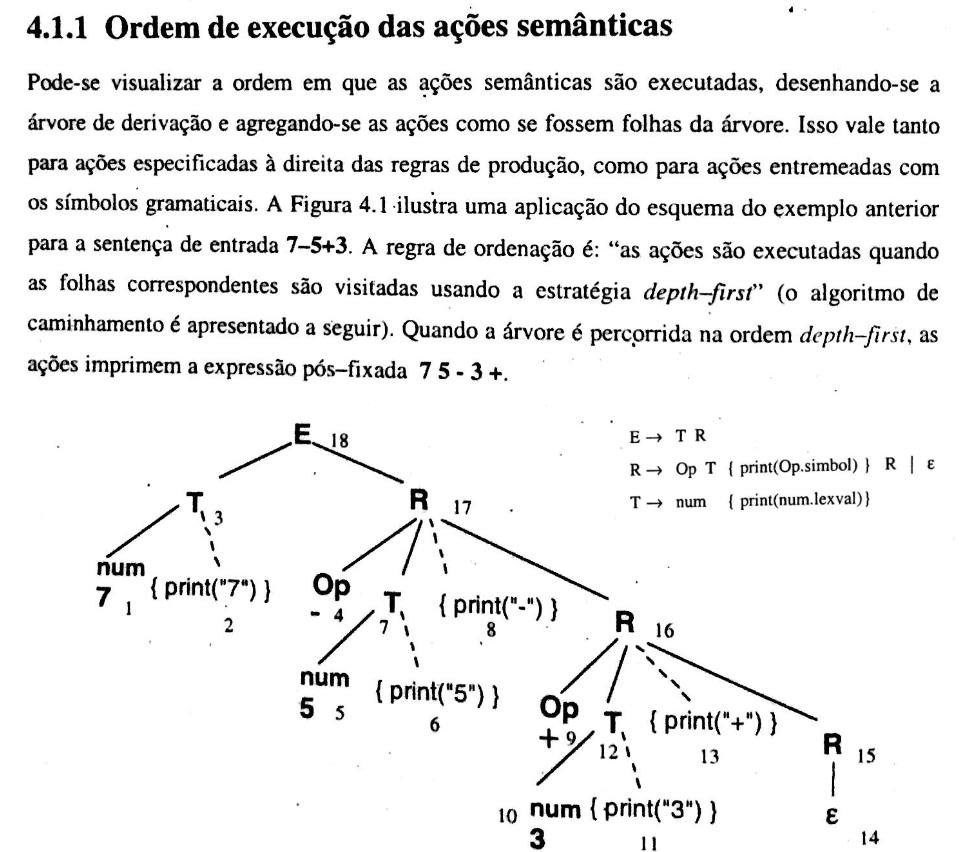
\includegraphics[scale=0.5]{images/arvore-traducao.png}\\
	\end{center}
	A aula seguiu explicando o exemplo da página 7 do fragmento do livro no arquivo \textit{3\_material...} que está no repositório.

\begin{verbatim}
Na GLC:
- Adicionar as produções:
		E::= E-T
		T::= T/F
	e respectivas ações semânticas

- Reconhecer a cadeia:
	8+((6/2-1)+2)=
----------------------------------------
GLC:            Ações semânticas:
	L::= E=  				{print (E.val)}
	E::= E1+T 			{E.val = E1.val + T.val}
	E::= T   				{E.val = T.val}
	T::= T1*F 			{T.val = T1.val * F.val}
	T::= F   				{T.val = F.val}
	F::= (E)  			{F.val = E.val}
	F::= id	  			{F.val = id.lexval}
	E::= E-T  			{E.val = E1.val - T.val}
	T::= T/F  			{T.val = T1.val / F.val}

	
	
Árvore:







E           |
|           |
id.        id.   id.   id.         id.         id.   id.         id.   id.
lex        lex   lex   lex         lex         lex   lex         lex   lex
=8         =(    =(    =6          =2          =1    =)          =2    =)
|           |     |     |           |           |     |           |     |
8     +     (     (     6     /     2     -     1     )     +     2     )     =
\end{verbatim}
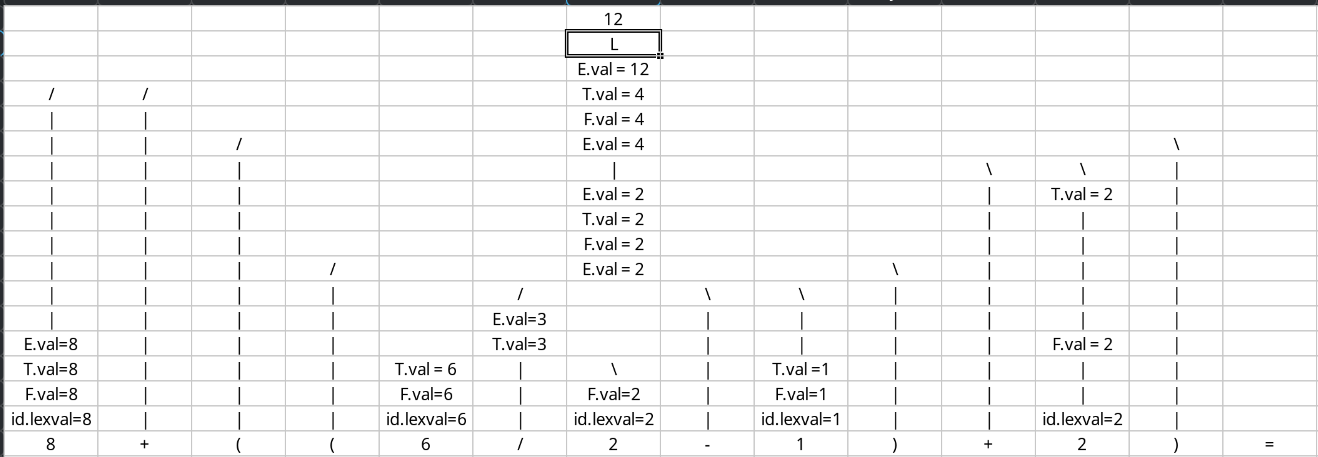
\includegraphics[scale=0.4]{images/arvore-calculadora.png}\\

	\subsection{Ações Semânticas}
		↓→ Tabela de Símbolos.

		Usamos ações semânticas para adicionar informações na tabela de símbolos.
		Tradução dirigida pela sintaxe, o conjunto de ações semânticas é chamado de esquemas de tradução.

		A execução dessas ações pode gerar ou interpretar código, armazenar informações na tabela de símbolos, emitir mensagens de erros, etc.

		\begin{itemize}
			\item esquemas de tradução
				\begin{itemize}
					\item declarações
					\item operações
				\end{itemize}
		\end{itemize}

O deslocamento é uma informação que é gerada a partir do reconhecimento sintático para dizer a partir de qual posição ifajof precisam ser geradas.
\begin{verbatim}
P::= MD
M::= \epsilon {desloc = 0}
D::= D, D
D::= id:T {addSb (id.nome, T.tipo, desloc); desloc = desloc+T.tam}
T::= int {T.tipo = int; T.tam=4}
T::= real {T.tipo = real; t.tam=8}
T::= array[num] of T1 {T.tipo = matriz(num.val, T1.tipo); T.tam=num.val*T1.tam}
T::= ^T1 {T.tipo = ponteiro (T1.tipo); T.tam=4}
\end{verbatim}
\newpage
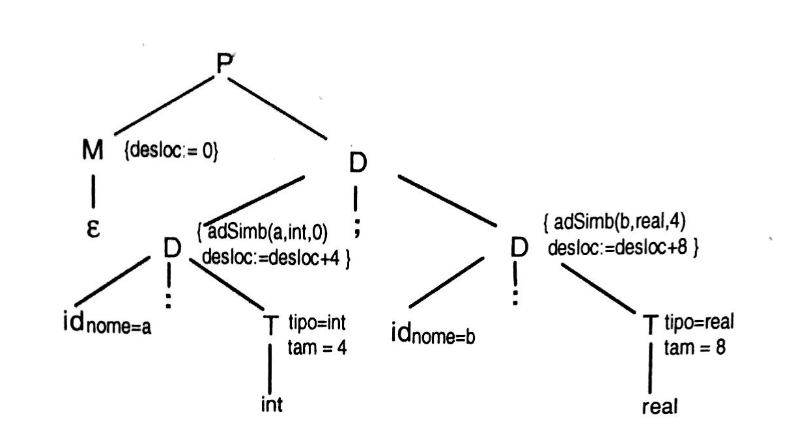
\includegraphics[scale=0.7]{images/arvore-derivacao-exemplo.png}\\
\textbf{Exemplo de arvore de derivação para "a: int; b: real"}.\\
\begin{verbatim}
	TS
	___________________________________
	| a, int, 0
	| b, real, 4
	desloc = _ _ 12
	         0 4

\end{verbatim}

\section{Geração de Código Intermediário}
	A árvore de derivação forma o \textbf{segmento de código}.


	A grande diferença entre o código intermediário e o código objeto final é que o intermediário não especifica detalhes da máquina alvo, tais como quais registradores serão usados, quais endereços de memória serão referenciados, etc...



	Temos uma gramática livre de contexto e uma expressão, precisamos adicionar ações semânticas para gerar o código intermediário. Fazer o reconhecimento e ver o que tem que ser feito. Adicionar as ações semânticas conforme subimos na árvore. Na saída vai ser armazenada como uma operação básica, no código intermediário será guardado o resultado temporário ($T.nome=geraTemp$). Adicionar 1-etc ao T na gramática quando o $T::=Txxx$ se T for derivado.


	\begin{itemize}
		\item intermediário
		\item 3 endereços
		\item independente da máquina
		\item instruções (arq)
	\end{itemize}

	Código intermediário.

	Simplifica a implementação do compilador.


	Tradução para outras máquinas.

	otimização

	1 passo a mais.

	\subsection{Código de 3 endereços}

\begin{verbatim}
	A = B op C
	A = op B
	A = B
	goto L
	if A oprel B goto L

	A= X+Y*Z

	T1 = 
	.
	.
	.
	.

	S::= id = E {S.cod=E.cod((gerocod(id.nome'='E.nome)}
	E::=E1+E2 {E.nome=geratemp;E.cod=E1.cod((E2.cod(
				                (geracod(E.nome'='e1.nome'+'E2.nome)}
	E::=E1*E2 {E.nome=geratemp;E.cod=E1.cod((E2.cod(
				                (geracod(E.nome'='e1.nome'+'E2.nome)}
	E::=(E1) {E.nome=E1.nome;E.cod=E1.cod}
	E::=id {E.nome=id.nome;E.cod=' '}
\end{verbatim}
	\subsection{Tarefa: gerar esquema de tradução para construir codigo intermediário adicionando código em saída}
\begin{verbatim}
	S::= id=E
	E::= E+T | E-T | T
	T::= T*F | T/F |F
	F::= (E) | id
\end{verbatim}

	\subsection{Otimização de código}
		\begin{itemize}
			\item tempo de compilação
				\begin{itemize}
					\item Desenvolvimento
					\item Execução de código
				\end{itemize}
			\item eliminar
				\begin{itemize}
					\item atribuições de redundância
					\item subexpressões comuns
					\item temporários desnecessários
				\end{itemize}
			\item mudar ordem de operações
			\item gerência de memória
		\end{itemize}

	\subsection{Representação Blocos Básicos por Grafo Acíclico Dirigido}
		\begin{itemize}
			\item folhas: operandos
			\item nodos: operadores
		\end{itemize}
		exemplo: $x = (a+b) * (a-b)$

	\subsection{Algoritmo de construção de Grafo Acíclico Dirigido}
		\begin{enumerate}
			\item Se $y \nexists$ no Grafo Acíclico Dirigido then cria folha $y$
			\item se $\exists$ nodo $op$ com folhas $y$ e $z$ then denommine de $x$ else cria nodo $x$.
		\end{enumerate}
	\textbf{Exemplo}

\begin{verbatim}
	T1 = a + b
	T2 = a - b
	T3 = T1 + T2
	T4 = a - c
	T5 = b - c
	T6 = T2 * T4
	T7 = T6 - T5
\end{verbatim}

\begin{center}
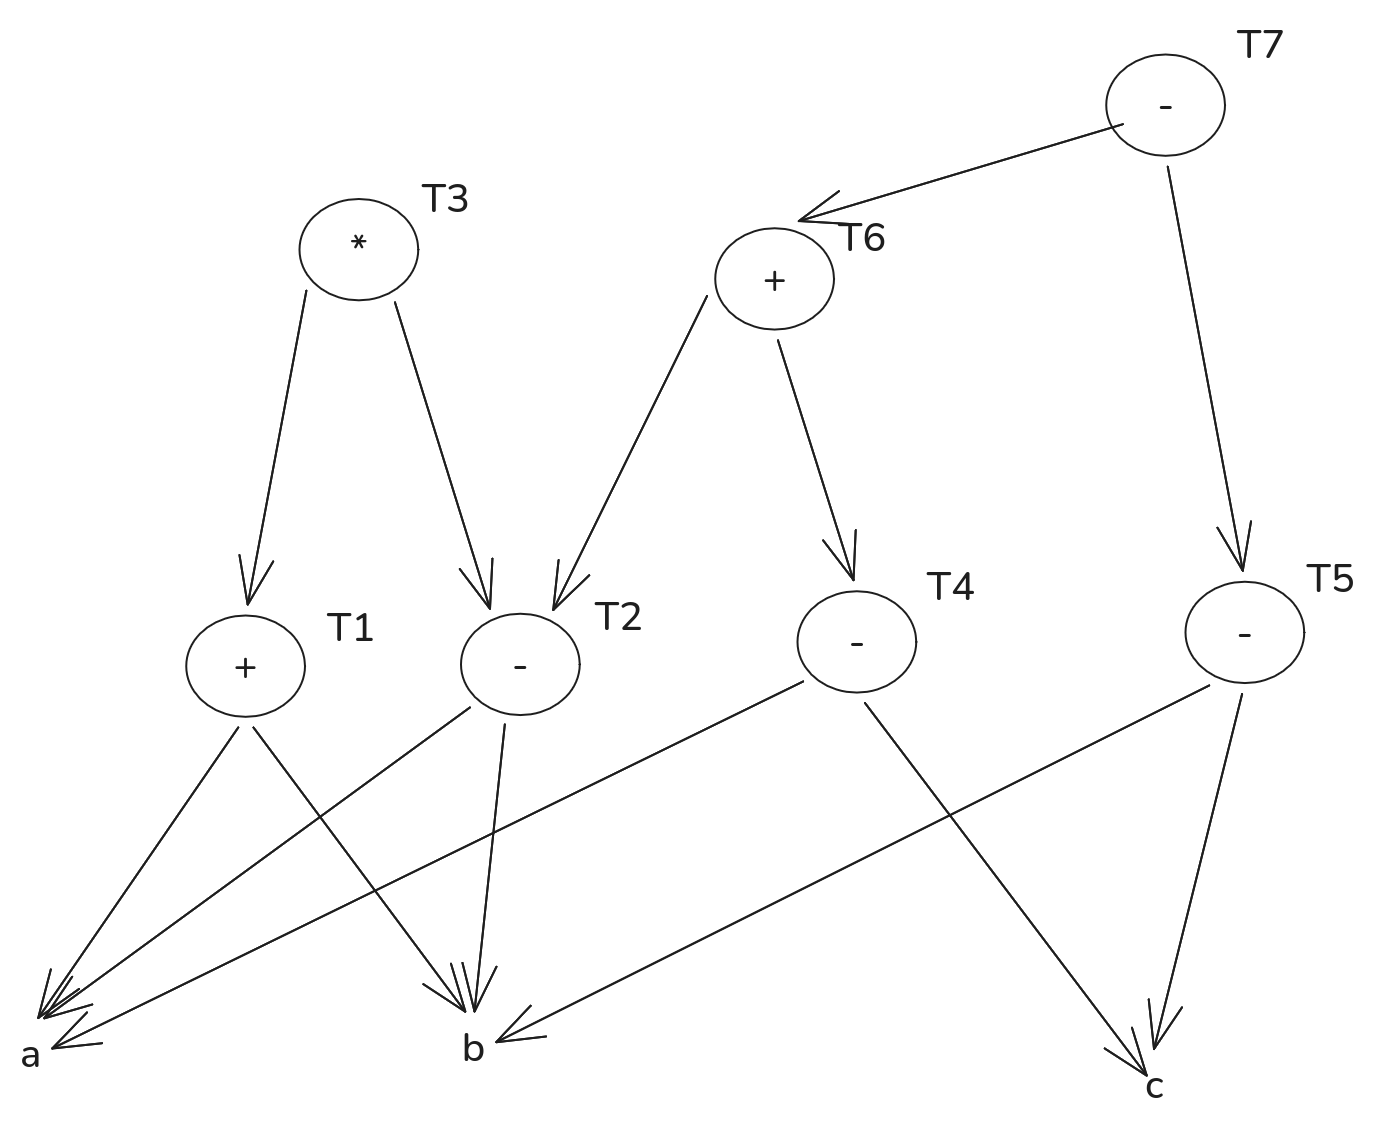
\includegraphics[scale=0.3]{images/GAD.png}
\end{center}

	\subsection{Sequência Otimizada de Execução}
		\begin{itemize}
			\item Faça $L=\o$
			\item Escolha nodo $n$ que $\nexists in L$
			\item se $\exists$ arestas incidentes em n then( se originou-se em nodos $\exists in L$ then $add$ $n$ $in$ $L$)
			\item se n é o último em L and aresta mais à esquerda originado em n incide em n e $\nexists$ em L and predecessores de n $\exists$ em L then add n em L

		\end{itemize}

\end{document}
